%%%%%%%%%%%%%%%%%%%%%%%%%%%%%%%%%%%%%%%%%%%%%%%%%%%%%%%%%%%%%%%%%%%%%%%%%%%%%%%%
% PREÁMBULO
% Este documento está configurado para ser compilado con pdflatex.
% Utiliza el estándar de artículo A4 con una sola columna.
%%%%%%%%%%%%%%%%%%%%%%%%%%%%%%%%%%%%%%%%%%%%%%%%%%%%%%%%%%%%%%%%%%%%%%%%%%%%%%%%
\documentclass[11pt, a4paper]{article}

% --- Codificación y Soporte de Idioma Español ---
\usepackage[utf8]{inputenc} % Permite escribir acentos y ñ directamente
\usepackage[T1]{fontenc}    % Codificación de fuentes moderna
\usepackage[spanish]{babel} % Soporte para español (títulos, guiones)

% --- Formato y Tipografía ---
\usepackage{times} % Fuente Times New Roman (común en reportes de ingeniería)
\usepackage[a4paper, margin=1in]{geometry} % Márgenes de 1 pulgada
\setlength{\parindent}{1em} % Indentación de párrafo
\setlength{\parskip}{0.5em} % Espacio entre párrafos

% --- Paquetes Esenciales ---
\usepackage{graphicx}   % Para insertar imágenes (tus capturas)
% Permitir cortes adecuados en URLs antes de cargar hyperref
\PassOptionsToPackage{hyphens}{url}
\usepackage[hidelinks]{hyperref} % Para URLs y referencias (sin cajas rojas)
% (url será cargado por hyperref con la opción 'hyphens')
\usepackage{caption}    % Mejor control sobre las captions de figuras
\usepackage{fancyhdr}   % Para cabeceras y pies de página

% --- Configuración de Cabecera ---
\pagestyle{fancy}
\fancyhf{} % Limpiar cabecera y pie
\fancyhead[L]{LIS-4052: Sistemas Distribuidos}
\fancyhead[R]{Actividad 4: RMI y gRPC}
\fancyfoot[C]{\thepage}
% Requerido por fancyhdr para evitar advertencia de altura de cabecera
\setlength{\headheight}{14pt}

%%%%%%%%%%%%%%%%%%%%%%%%%%%%%%%%%%%%%%%%%%%%%%%%%%%%%%%%%%%%%%%%%%%%%%%%%%%%%%%%
% BLOQUE DE TÍTULO
%%%%%%%%%%%%%%%%%%%%%%%%%%%%%%%%%%%%%%%%%%%%%%%%%%%%%%%%%%%%%%%%%%%%%%%%%%%%%%%%
\title{Implementación y Análisis de un Sistema de Subastas Distribuido con Java RMI y gRPC}

\author{
  \textbf{Miembros del Equipo:}\\
  Camila García Álvarez\\
  Celeste Isabel Alonso García\\
  Jesús Álvarez Sombrerero
  \vspace{1em} \\
  \textit{Departamento de Computación, Electrónica y Mecatrónica}\\
  \textit{Universidad de las Américas Puebla (UDLAP)}
}

\date{26 de octubre de 2025 \\ \vspace{1em}
    \textbf{Materia:} LIS–4052 Sistemas Distribuidos \\
    \textbf{Profesor:} José Luis Zechinelli Martini
}

%%%%%%%%%%%%%%%%%%%%%%%%%%%%%%%%%%%%%%%%%%%%%%%%%%%%%%%%%%%%%%%%%%%%%%%%%%%%%%%%
% DOCUMENTO
%%%%%%%%%%%%%%%%%%%%%%%%%%%%%%%%%%%%%%%%%%%%%%%%%%%%%%%%%%%%%%%%%%%%%%%%%%%%%%%%
\begin{document}

\maketitle
\thispagestyle{empty} % Sin cabecera/pie en la página del título

\begin{abstract}
\textbf{Resumen:} Este reporte detalla el diseño, migración e implementación de una aplicación de subastas, transformándola de una arquitectura centralizada (Modelo-Vista-Controlador) a un sistema distribuido. Siguiendo los lineamientos de la Actividad 4, se implementaron dos soluciones paralelas utilizando distintas tecnologías de middleware: Java Remote Method Invocation (RMI) y gRPC. El desafío principal de la práctica, la sincronización de estado en tiempo real entre múltiples clientes, se resolvió exitosamente mediante la implementación del patrón observador. En RMI, esto se logró a través de un sistema de callbacks remotos, y en gRPC, mediante el uso de server-side streaming. El reporte presenta el diseño de ambas soluciones, un análisis de los datos obtenidos durante la experimentación (basado en la rúbrica SO6) y una comparación técnica de las ventajas y desventajas de RPC, RMI y gRPC para este caso de uso.
\end{abstract}

\newpage
\tableofcontents % Añadir una tabla de contenido
\newpage

% --- Sección 1: Objetivo ---
\section{Objetivo de la Práctica}
\label{sec:objetivo}

El objetivo de esta práctica es doble. Primero, revisar y aplicar los procedimientos necesarios para construir una aplicación distribuida partiendo de una versión centralizada, utilizando dos tecnologías de middleware clave: Java RMI y gRPC.

Segundo, y de manera fundamental, proponer e implementar una estrategia de software robusta para resolver el problema de la falta de sincronización de datos entre múltiples clientes. Específicamente, se debe asegurar que cuando un usuario propone un nuevo precio (una oferta) por un producto, las vistas de todos los demás clientes conectados se actualicen automáticamente sin requerir una acción manual (como presionar "Obtener lista").

Como entregable final, se debe preparar este reporte demostrando la capacidad del equipo para (acorde a la rúbrica SO6):
\begin{itemize}
    \item Diseñar y llevar a cabo una experimentación adecuada.
    \item Analizar e interpretar los datos obtenidos (logs, comportamiento de la GUI).
    \item Utilizar el juicio de ingeniería para sacar conclusiones válidas.
\end{itemize}

% --- Sección 2: Diseño de la Solución ---
\section{Diseño de la Solución}
\label{sec:diseno}

La aplicación original proveída sigue el patrón Modelo-Vista-Controlador (MVC). La \texttt{SubastaVista} maneja la GUI de Swing, \texttt{SubastaModelo} contiene la lógica de negocio y el estado (listas de usuarios, productos y ofertas), y \texttt{SubastaControlador} actúa como puente.

\subsection{Arquitectura Distribuida}
La migración a un sistema distribuido se basa en identificar el \texttt{SubastaModelo} como el componente a ser centralizado y servido.
\begin{itemize}
    \item \textbf{Servidor:} La lógica de \texttt{SubastaModelo} se convierte en el servicio remoto. Es el único que mantiene el estado verdadero del sistema.
    \item \textbf{Cliente:} Las clases \texttt{SubastaVista} y \texttt{SubastaControlador} permanecen en la máquina cliente. El \texttt{SubastaControlador} es modificado para, en lugar de invocar métodos locales del modelo, realizar llamadas remotas (RMI o gRPC) al servidor.
\end{itemize}

\subsection{Estrategia de Sincronización: Patrón Observador (Push)}
El problema central es que una llamada remota (ej. \texttt{agregaOferta}) de un Cliente A al Servidor, no tiene forma de notificar al Cliente B. La solución implementada es el \textbf{Patrón Observador (Observer Pattern)}.

El Servidor actúa como el "Sujeto" (Subject) y los Clientes actúan como "Observadores" (Observers).
\begin{enumerate}
    \item \textbf{Registro:} Cuando un cliente se conecta, no solo se registra como usuario, sino que también se "suscribe" a las actualizaciones del servidor.
    \item \textbf{Lista de Observadores:} El servidor mantiene una lista de todos los observadores suscritos (es decir, todos los clientes conectados).
    \item \textbf{Notificación (Push):} Cuando ocurre un evento de cambio de estado (como \texttt{agregaProductoALaVenta} o \texttt{agregaOferta}), el servidor itera sobre su lista de observadores y les "empuja" (push) una notificación de que algo ha cambiado.
    \item \textbf{Actualización del Cliente:} El cliente, al recibir esta notificación asíncrona, es instruido para recargar su catálogo de productos desde el servidor, refrescando así su GUI.
\end{enumerate}

Este patrón se implementó de forma idiomática en cada tecnología:
\begin{itemize}
    \item \textbf{En RMI:} Se implementó mediante \textbf{Callbacks}. Se define una nueva interfaz remota, \texttt{ClienteCallbackRMI}, que el cliente implementa. El cliente envía su propio stub (referencia remota a sí mismo) al servidor, el cual lo almacena en un \texttt{Vector}. Cuando hay una actualización, el servidor invoca el método \texttt{notificarActualizacion()} en cada stub de cliente en su lista.
    \item \textbf{En gRPC:} Se implementó mediante \textbf{Server-side Streaming}. Se define un RPC en el archivo \texttt{.proto} llamado \texttt{suscribirseNotificaciones} que retorna un \texttt{stream} de mensajes. El cliente llama a este método una vez y mantiene la conexión abierta. El servidor almacena el objeto \texttt{StreamObserver} del cliente. Cuando hay una actualización, el servidor llama a \texttt{onNext()} en cada \textit{observer} de su lista, enviando un mensaje de notificación por el stream.
\end{itemize}

% --- Sección 3: Pasos de Desarrollo ---
\section{Principales Pasos para Desarrollar la Solución}
\label{sec:pasos}

\subsection{Implementación RMI}
\begin{enumerate}
    \item \textbf{Definición de Interfaces:} Se crearon dos interfaces \texttt{java.rmi.Remote}: \texttt{SubastaServidorRMI} (para las operaciones principales) y \texttt{ClienteCallbackRMI} (para la notificación).
    \item \textbf{Serialización:} Las clases de datos \texttt{InformacionProducto} e \texttt{InformacionOferta} fueron modificadas para implementar \texttt{java.io.Serializable}.
    \item \textbf{Implementación del Servidor:} Se creó \texttt{SubastaModeloRMI} extendiendo \texttt{UnicastRemoteObject} e implementando la interfaz del servidor. Se añadió un \texttt{Vector<ClienteCallbackRMI>} para gestionar los callbacks.
    \item \textbf{Implementación del Cliente:} Se modificó \texttt{ClienteRMI} para buscar el stub del servidor en \texttt{rmiregistry}. Se implementó la interfaz de callback y se registró en el servidor al conectarse. El \texttt{SubastaControladorRMI} fue adaptado para realizar llamadas RMI.
\end{enumerate}

\subsection{Implementación gRPC}
\begin{enumerate}
    \item \textbf{Definición de Contrato (IDL):} Se creó el archivo \texttt{subasta.proto} definiendo los mensajes (ej. \texttt{OfertaRequest}) y los servicios (\texttt{rpc AgregaOferta}). Crucialmente, se definió el stream: \texttt{rpc suscribirseNotificaciones(Empty) returns (stream NotificacionUpdate);}.
    \item \textbf{Generación de Código:} Se utilizó Gradle y el plugin de \texttt{protobuf} para generar el código stub de Java.
    \item \textbf{Implementación del Servidor:} Se creó \texttt{SubastaServicioImpl} extendiendo la clase base generada por gRPC. La lógica del modelo se migró aquí, incluyendo un \texttt{ConcurrentHashMap} para almacenar los \texttt{StreamObserver} de los clientes suscritos.
    \item \textbf{Implementación del Cliente:} Se creó \texttt{ClienteGPRC}, que instancia un \texttt{ManagedChannel} para conectarse al servidor. El \texttt{SubastaControladorGPRC} utiliza el stub bloqueante para acciones (como ofertar) y el stub asíncrono para suscribirse al stream de notificaciones en un hilo separado.
\end{enumerate}

% --- Sección 4: Seguridad ---
\section{Aspectos de Seguridad en el Desarrollo}
\label{sec:seguridad}

En un sistema distribuido, la seguridad no es opcional.
\begin{itemize}
    \item \textbf{RMI:} La seguridad en RMI es compleja y anticuada. Requiere un \texttt{SecurityManager} y archivos de políticas (\texttt{.policy}) para definir permisos. La funcionalidad de \texttt{codebase} (descarga de clases remotas) es una vulnerabilidad conocida si no se configura adecuadamente. La comunicación por defecto no está cifrada.
    \item \textbf{gRPC:} gRPC está construido sobre HTTP/2 y promueve la seguridad como una característica central. Se integra nativamente con SSL/TLS para cifrar toda la comunicación entre cliente y servidor. Para las pruebas de esta práctica, se utilizó \texttt{usePlaintext()}, pero en un entorno de producción, habilitar el cifrado es trivial. Además, gRPC soporta mecanismos de autenticación por llamada, como tokens (ej. JWT).
\end{itemize}

% --- Sección 5: Presentación de Datos e Interfaz ---
\section{Presentación de los Datos: Interfaz del Sistema}
\label{sec:interfaz}

La interfaz de usuario (\texttt{SubastaVista.java}) no sufrió modificaciones visuales. Sigue presentando las cuatro zonas funcionales descritas en las instrucciones:
\begin{enumerate}
    \item \textbf{Iniciar sesión:} Captura del nombre de usuario.
    \item \textbf{Poner producto a la venta:} Nombre del producto y precio inicial.
    \item \textbf{Obtener lista de productos:} Lista de productos y precio actual.
    \item \textbf{Hacer una oferta:} Monto ofrecido.
\end{enumerate}

El cambio fundamental no es visual, sino funcional. Gracias a la solución de sincronización (callback/stream), la "Zona de lista de productos" y el "Precio actual" ahora se actualizan de forma reactiva. Cuando un cliente B realiza una oferta, el servidor envía la notificación. El cliente A recibe esta notificación y su controlador es instruido para recargar la lista y el precio, reflejando el nuevo estado del sistema sin intervención del usuario.

% --- Sección 6: Demostración y Análisis de Ejemplos ---
\section{Demostración de Ejemplos y Análisis (SO6)}
\label{sec:demo}

Acorde a la rúbrica SO6 ("Diseño de experimentos", "Análisis de datos"), se diseñó un experimento para validar la funcionalidad de ambas implementaciones, específicamente la solución al problema de sincronización.

\subsection{Experimento RMI (Java RMI)}
El experimento consistió en lanzar un servidor y dos clientes (Cliente 1: "Jesus", Cliente 2: "OtroUsuario").
\begin{itemize}
    \item \textbf{Paso 1: Venta (Cliente 1):} El Cliente 1 ("Jesus") se conecta y pone a la venta un "Libro" por 135 (ver Fig. \ref{fig:rmi_vender_gui}).
    \item \textbf{Paso 2: Notificación (Cliente 1):} La terminal del Cliente 1 (Fig. \ref{fig:rmi_vender_term}) muestra "Poniendo a la venta: Libro" e inmediatamente "CALLBACK RECIBIDO: El precio de 'Nuevo producto: Libro' ahora es 135.0".
    \item \textbf{Paso 3: Oferta (Cliente 2):} El Cliente 2 se conecta, obtiene la lista (viendo "Libro") y realiza una oferta de 135 (ver Fig. \ref{fig:rmi_oferta_gui} y \ref{fig:rmi_oferta_term}).
\end{itemize}

\begin{figure}[h!]
    \centering
    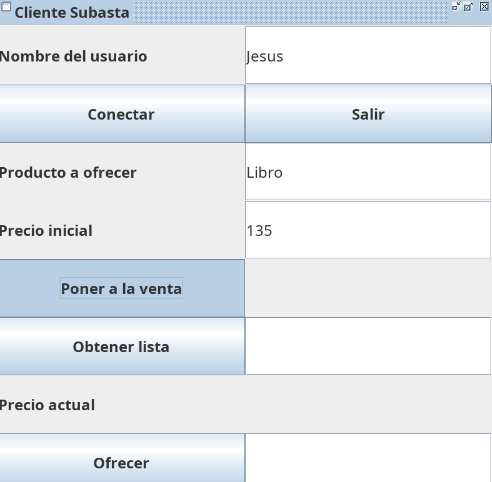
\includegraphics[width=0.7\linewidth]{media/rmi-screenshots/Sell-Item-Client1.png}
    \caption{RMI: Cliente 1 ("Jesus") poniendo a la venta un "Libro" por 135.}
    \label{fig:rmi_vender_gui}
\end{figure}

\begin{figure}[h!]
    \centering
    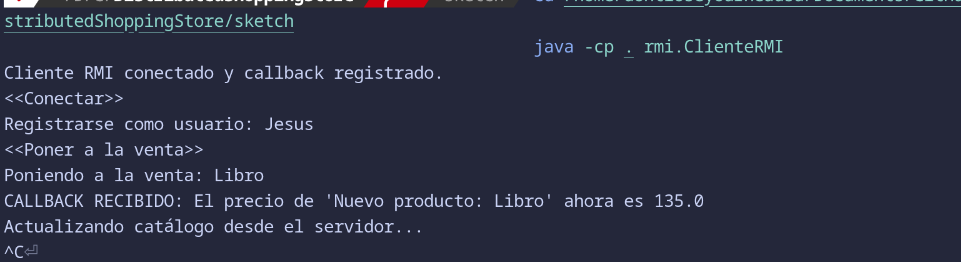
\includegraphics[width=0.9\linewidth]{media/rmi-screenshots/Sell-Item-Terminal-Client-1.png}
    \caption{RMI: Terminal del Cliente 1. La línea "CALLBACK RECIBIDO" demuestra que el servidor notificó exitosamente al cliente sobre el nuevo producto.}
    \label{fig:rmi_vender_term}
\end{figure}

\begin{figure}[h!]
    \centering
    \begin{minipage}{0.48\textwidth}
        \centering
        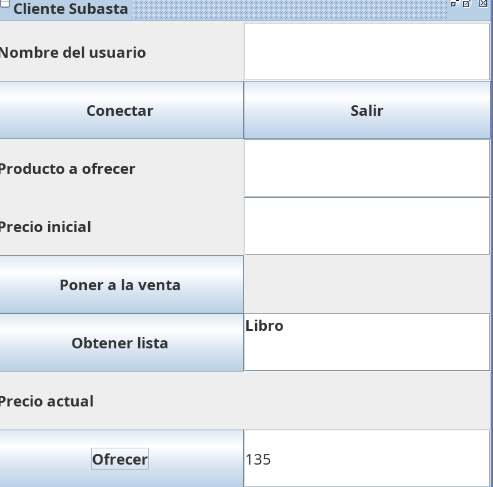
\includegraphics[width=\linewidth]{media/rmi-screenshots/Offer-Client2.png}
        \caption{RMI: Cliente 2 visualiza el "Libro" y prepara una oferta de 135.}
        \label{fig:rmi_oferta_gui}
    \end{minipage}\hfill
    \begin{minipage}{0.48\textwidth}
        \centering
        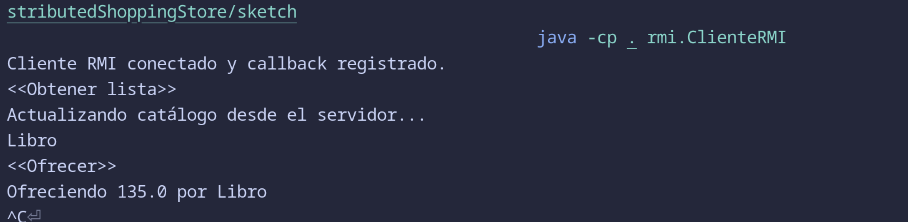
\includegraphics[width=\linewidth]{media/rmi-screenshots/Offer-Terminal-Client2.png}
        \caption{RMI: Terminal del Cliente 2, registrando la acción "Ofrecer".}
        \label{fig:rmi_oferta_term}
    \end{minipage}
\end{figure}

\textbf{Análisis de Datos (RMI):} El dato más importante es la línea "CALLBACK RECIBIDO" en la Fig. \ref{fig:rmi_vender_term}. Demuestra que el patrón observador fue implementado correctamente. El servidor notificó exitosamente al cliente (en este caso, al mismo cliente que realizó la acción) sobre el cambio de estado. Esto confirma que el mecanismo de "push" funciona.

\subsection{Experimento gRPC}
El experimento consistió en lanzar un servidor y dos clientes (Cliente 1: "Camila", Cliente 2: "Celeste"). La Figura \ref{fig:grpc_full} captura la totalidad del experimento.

\begin{figure}[h!]
    \centering
    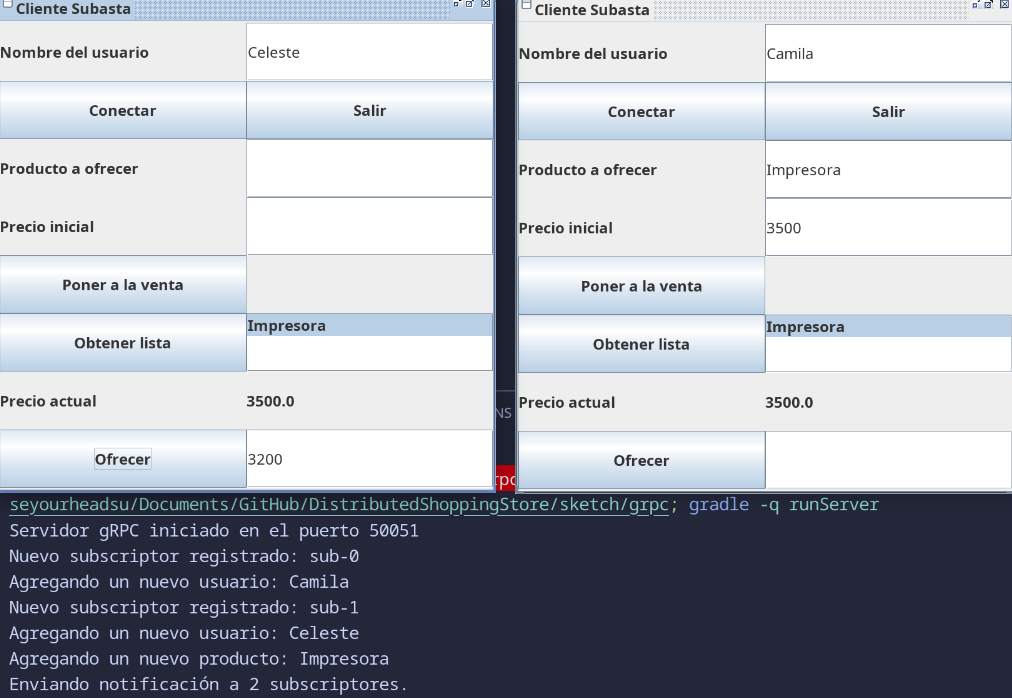
\includegraphics[width=1.0\linewidth]{media/grpc-screenshots/Two-Clients+Server-Output.png}
    \caption{gRPC: Demostración completa con servidor y dos clientes ("Celeste" y "Camila").}
    \label{fig:grpc_full}
\end{figure}

\textbf{Análisis de Datos (gRPC):} La Fig. \ref{fig:grpc_full} es una demostración completa de la solución de sincronización (acorde al nivel 4 de la rúbrica SO6 "Design of experiments"):
\begin{enumerate}
    \item \textbf{Servidor (Terminal inferior):} El servidor inicia ("Servidor gRPC iniciado").
    \item \textbf{Conexión Cliente 1:} El servidor registra "Nuevo subscriptor registrado: sub-0" y "Agregando un nuevo usuario: Camila".
    \item \textbf{Conexión Cliente 2:} El servidor registra "Nuevo subscriptor registrado: sub-1" y "Agregando un nuevo usuario: Celeste".
    \item \textbf{Acción (Cliente 1 "Camila"):} La GUI de Camila (derecha) muestra que está poniendo a la venta una "Impresora" por "3500".
    \item \textbf{Notificación (Servidor):} El servidor registra la acción "Agregando un nuevo producto: Impresora" e inmediatamente "Enviando notificación a 2 subscriptores."
    \item \textbf{Resultado (Cliente 2 "Celeste"):} La GUI de Celeste (izquierda) muestra "Impresora" en su lista y "3500.0" como precio actual, \textit{sin que ella haya realizado ninguna acción} más que conectarse.
\end{enumerate}
Este experimento valida inequívocamente que el stream de gRPC notificó exitosamente al Cliente 2 sobre una acción realizada por el Cliente 1, resolviendo el problema central de la práctica.

% --- Sección 7: Análisis Comparativo ---
\section{Análisis y Comparación: RPC, RMI y gRPC}
\label{sec:comparacion}

Como solicita la práctica, se presenta una comparación de las tecnologías.

\begin{itemize}
    \item \textbf{RPC (Tradicional):}
    \begin{itemize}
        \item \textbf{Ventajas:} Es el concepto más simple de llamada a procedimiento remoto. Es agnóstico al lenguaje (si usa un IDL como XDR).
        \item \textbf{Desventajas:} Es un paradigma puramente síncrono de solicitud-respuesta. Resolver el problema de sincronización de esta práctica requeriría \textit{polling} (el cliente pregunta al servidor "¿hay cambios?" cada segundo), lo cual es altamente ineficiente, genera alta latencia y no escala.
    \end{itemize}
    
    \item \textbf{Java RMI (Usado):}
    \begin{itemize}
        \item \textbf{Ventajas:} Integración nativa y simple con el lenguaje Java. Permite pasar objetos Java serializables completos. El patrón de callback es una solución natural y elegante en un ecosistema puramente Java.
        \item \textbf{Desventajas:} Es una tecnología legada y monolítica, limitada exclusivamente a Java. Su configuración (\texttt{rmiregistry}, \texttt{codebase}, archivos de políticas) es considerada anticuada y verbosa.
    \end{itemize}
    
    \item \textbf{gRPC (Usado):}
    \begin{itemize}
        \item \textbf{Ventajas:} Es una tecnología moderna de alto rendimiento (basada en HTTP/2 y Protocol Buffers). Es completamente agnóstica al lenguaje, definida por un contrato \texttt{.proto}. Su soporte nativo para \textbf{streaming} (unidireccional y bidireccional) está diseñado precisamente para casos de uso como este, permitiendo una comunicación asíncrona y reactiva de forma eficiente.
        \item \textbf{Desventajas:} Requiere un paso de compilación/generación de código. La gestión de la comunicación asíncrona (streams, observadores) añade una capa de complejidad al código cliente en comparación con una simple llamada de RMI.
    \end{itemize}
\end{itemize}

% --- Sección 8: Conclusiones ---
\section{Conclusiones (Síntesis SO6)}
\label{sec:conclusiones}

Los objetivos de la práctica se han cumplido en su totalidad. Se logró migrar exitosamente la aplicación MVC centralizada a dos arquitecturas distribuidas funcionales.

La \textit{síntesis de la información} (rúbrica SO6) obtenida de los experimentos nos permite concluir que el problema de sincronización de estado fue resuelto exitosamente en ambas plataformas. La estrategia del patrón observador fue validada: los callbacks de RMI y los streams de gRPC demostraron ser mecanismos eficaces para "empujar" (push) las actualizaciones de estado a los clientes en tiempo real, como se evidencia en la Fig. \ref{fig:rmi_vender_term} y Fig. \ref{fig:grpc_full}.

Utilizando el \textit{juicio de ingeniería} (rúbrica SO6), se concluye que gRPC es la solución tecnológicamente superior. Aunque RMI fue funcional y elegante dentro de su ecosistema cerrado, gRPC ofrece una solución más robusta, de mayor rendimiento e interoperable, cuyo soporte nativo para streaming se alinea perfectamente con los requisitos de las aplicaciones distribuidas modernas y reactivas.

\newpage
% --- Anexo para Puntos Extra ---
\appendix

\section{Anexo: DECIMAS EXTRAS (Implementación RMI y gRPC)}
\label{sec:anexo}

Para la obtención de las décimas extras, el equipo implementó la solución completa en \textbf{ambas} plataformas (RMI y gRPC), no solo en una. El diseño y la implementación de ambas se describen en las Secciones \ref{sec:diseno} y \ref{sec:pasos} de este reporte.

Las siguientes capturas de pantalla, analizadas en la Sección \ref{sec:demo}, sirven como evidencia de la correcta implementación y funcionamiento de ambas soluciones, cumpliendo así con los requisitos para la puntuación adicional.

\subsection{Evidencia de Implementación RMI}

\begin{figure}[h!]
    \centering
    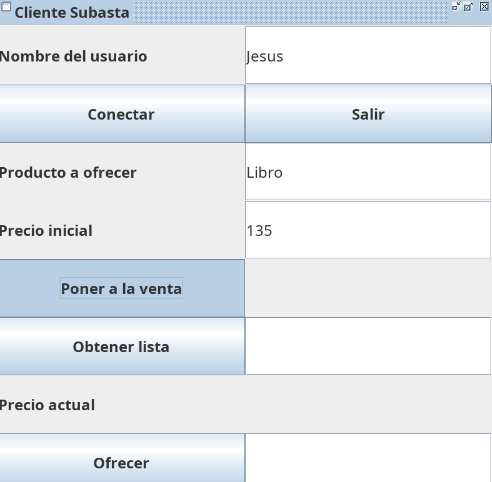
\includegraphics[width=0.7\linewidth]{media/rmi-screenshots/Sell-Item-Client1.png}
    \caption{Evidencia RMI: Cliente 1 registrando un producto.}
\end{figure}

\begin{figure}[h!]
    \centering
    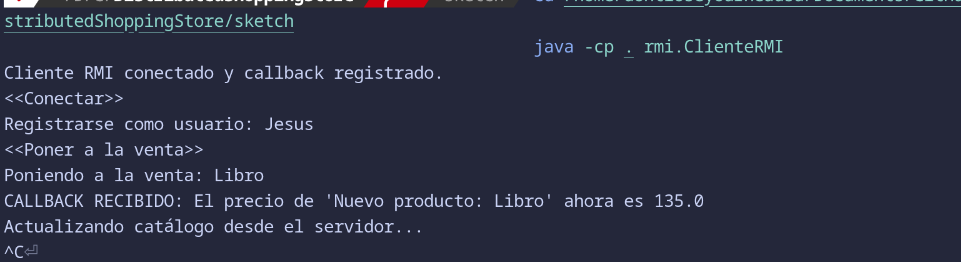
\includegraphics[width=0.9\linewidth]{media/rmi-screenshots/Sell-Item-Terminal-Client-1.png}
    \caption{Evidencia RMI: Terminal del Cliente 1 confirmando la recepción de un \textbf{callback} del servidor.}
\end{figure}

\subsection{Evidencia de Implementación gRPC}

\begin{figure}[h!]
    \centering
    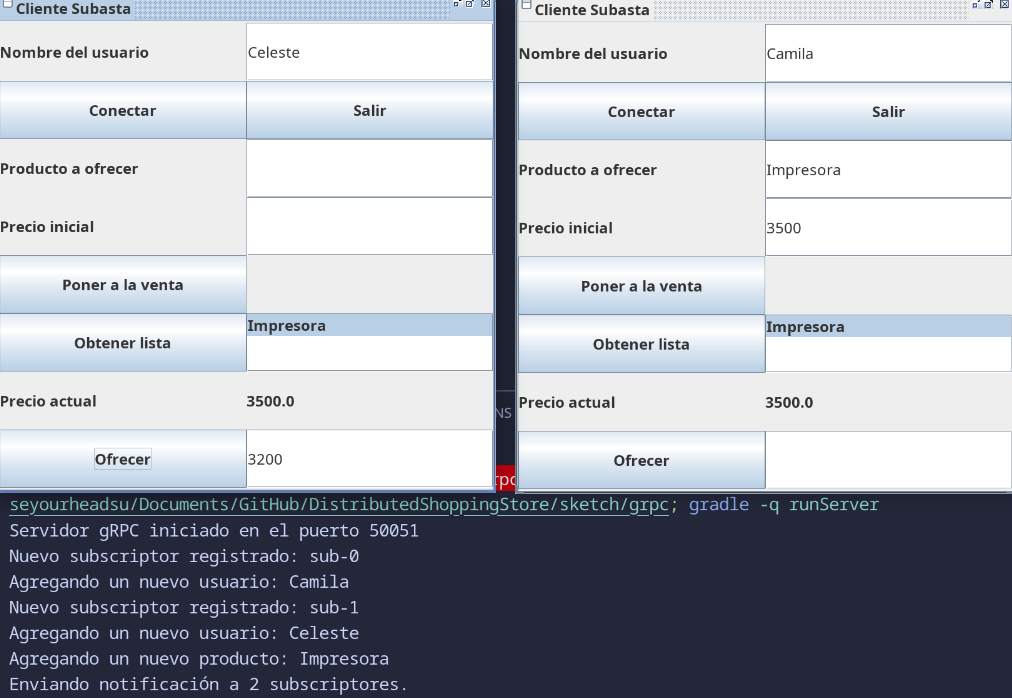
\includegraphics[width=1.0\linewidth]{media/grpc-screenshots/Two-Clients+Server-Output.png}
    \caption{Evidencia gRPC: El servidor (abajo) registra dos subscriptores (Camila, Celeste) y les \textbf{envía una notificación} (stream) tras el registro de un producto, actualizando la GUI del cliente observador (izquierda).}
\end{figure}


% --- Referencias ---
\newpage

\begin{thebibliography}{9}

\bibitem{tanenbaum}
A. S. Tanenbaum and M. Van Steen,
\textit{Distributed Systems: Principles and Paradigms (4th Edition)}.
Pearson, 2024.

\bibitem{coulouris}
G. Coulouris, J. Dollimore, T. Kindberg, and G. Blair,
\textit{Distributed Systems: Concepts and Design (5th Edition)}.
Addison-Wesley, 2011.

\bibitem{grpc_docs}
The gRPC Authors, "gRPC Documentation: Core Concepts, Architecture and Lifecycle."
\url{https://grpc.io/docs/what-is-grpc/core-concepts/}
[Consultado: 25 de octubre de 2025].

\bibitem{oracle_rmi}
Oracle Corporation, "Java RMI Documentation: An Overview."
\url{https://docs.oracle.com/javase/8/docs/technotes/guides/rmi/index.html}
[Consultado: 25 de octubre de 2025].

\end{thebibliography}

\end{document}
